\documentclass[tikz]{standalone}
\usepackage{amsmath,amssymb,multirow}
\usetikzlibrary{shapes.misc, positioning,automata,arrows,calc,fit}
\tikzset{VertexStyle/.style = {draw,circle,thick,
		minimum size=1cm,
		font=\Large\bfseries},thick} 
\usepackage{booktabs}
\begin{document}
  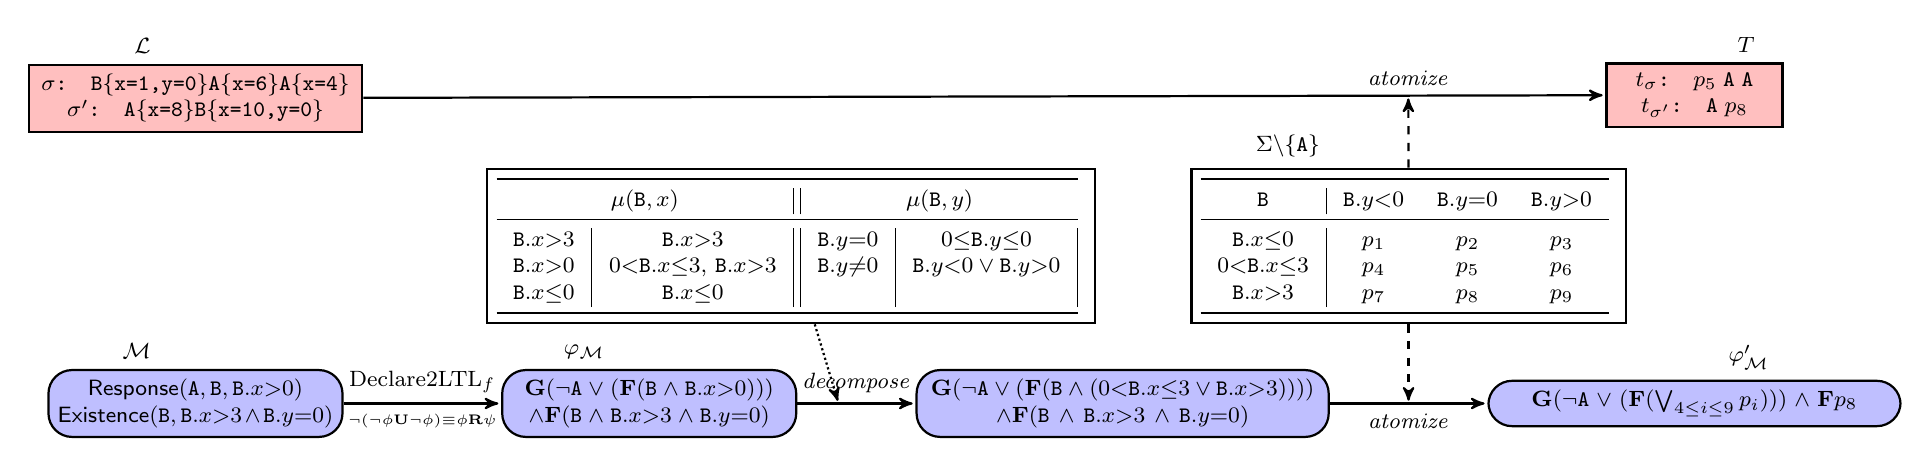
\begin{tikzpicture}[->,>=stealth',shorten >=1pt,thick,initial text=$ $,align=center,node distance=5mm,font=\footnotesize]
\thickmuskip=0mu
%% Input
\node (Clause)  [fill=blue!25,text width=3.5cm,rounded corners=.3cm,draw=black,label=above left:{$\mathcal{M}$}] 
				{$\mathsf{Response}(\texttt{A},\texttt{B},\;\texttt{B}.x>0)$\\
				 $\mathsf{Existence}(\texttt{B},\; \texttt{B}.x>3\wedge \texttt{B}.y=0)$};
			 
%% Straightforward translation
%\node (LTLf1) 
%				[right=2cm of Clause,fill=blue!25,text width=3cm,rounded corners=.3cm,draw=black] 
%				{$\square(\texttt{A}\Rightarrow \lozenge(\texttt{B}\wedge \texttt{B}.x>0))$\\
%				 $\lozenge(\texttt{B}\wedge \texttt{B}.x>3\wedge \texttt{B}.y=0)$};
				
%% Conversion to NNF				
\node (LTLf2) 	[right=2cm of Clause,fill=blue!25,text width=3.5cm,rounded corners=.3cm,draw=black,label=above left:{$\varphi_{\mathcal{M}}$}] 
				{$\mathbf{G} (\neg\texttt{A} \vee (\mathbf{F}\;(\texttt{B}\wedge \texttt{B}.x>0)))$\\
				 $\wedge\;\;\mathbf{F}\;(\texttt{B}\wedge \texttt{B}.x>3\wedge \texttt{B}.y=0)$};
\draw[->] (Clause) -- (LTLf2) node[midway,above] {Declare2LTL$_f$} node[midway,below] {${\scriptscriptstyle \neg(\neg\phi\mathbf{U}\neg\phi)\equiv\phi\mathbf{R}\psi}$};
%\draw[->] (LTLf1) --  (LTLf2) node[midway,above] {\textit{nnf}};

%% Data predicates decomposition
\node (LTLf3) 	[right=1.5cm of LTLf2,fill=blue!25,text width=5cm,rounded corners=.3cm,draw=black] 
				{$ \mathbf{G} (\neg\texttt{A} \vee (\mathbf{F}\;(\texttt{B}\wedge \left(0<\texttt{B}.x\leq 3\vee \texttt{B}.x>3\right))))$\\
				 $\wedge\;\;\mathbf{F}\;(\texttt{B}\wedge \texttt{B}.x>3\wedge \texttt{B}.y=0)$};
\draw[->] (LTLf2) --  (LTLf3) node[midway,above] {\textit{decompose}};

\node (tab1) [ shape=rectangle,draw] at ($(LTLf2)!0.3!(LTLf3)+(0,2)$) {
	\begin{tabular}{c|c||c|c|}
	\toprule
	\multicolumn{2}{c||}{$\mu(\texttt{B},x)$} & \multicolumn{2}{c}{$\mu(\texttt{B},y)$}\\
	\midrule
	$\texttt{B}.x>3$      & $\texttt{B}.x>3$ & $\texttt{B}.y=0$ & $0\leq \texttt{B}.y\leq 0$\\
	$\texttt{B}.x> 0$ & $0<\texttt{B}.x\leq 3$, $ \texttt{B}.x>3$ & $\texttt{B}.y\neq 0$ & $\texttt{B}.y<0\vee \texttt{B}.y>0$\\
	$\texttt{B}.x\leq 0$ & $ \texttt{B}.x\leq 0$ & & \\
	\bottomrule
	\end{tabular}
};
\draw[->,densely dotted] (tab1) -- ($(LTLf2)!0.4!(LTLf3)$);

\node (LTLf4) 	[right=2cm of LTLf3,fill=blue!25,text width=5cm,rounded corners=.3cm,draw=black,label=above right:{$\varphi_{\mathcal{M}}'$}] 
				{$\mathbf{G}(\neg\texttt{A}\vee(\mathbf{F}(\bigvee_{4\leq i\leq9}p_i)))\wedge\mathbf{F} p_8$};

\node (Traces) [fill=red!25,text width=4cm,draw=black,above=3cm of Clause,label=above left:{$\mathcal{L}$}] 
			   {$\sigma$\texttt{:\quad B\{x=1,y=0\}A\{x=6\}A\{x=4\}}\\
				$\sigma'$\texttt{:\quad A\{x=8\}B\{x=10,y=0\}}};

\node (CTraces) [fill=red!25,text width=2cm,draw=black,above=3.2cm of LTLf4,label=above right:{$T$}] 
                {$t_\sigma$\texttt{:\quad $p_5$\;\texttt{A\;A}}\\
                 $t_{\sigma'}$\texttt{:\quad A}\;$p_8$};

%\node[state,initial] (SA) at ($(LTLf4)-(1.3,3.5)$) {$s_1$};
%\path (SA) edge[loop] node[midway,above] (W1) {$\Sigma\backslash\{p_1,p_3\}$} (SA);
%\node[state,accepting,right =2cm of SA] (ST) {$s_2$};
%\path (ST) edge[loop] node[midway,above] (W2) {$\Sigma\backslash\{p_3\}$} (ST);
%\draw[->] (SA) -- (ST) node[midway,above] {$\{p_1\}$};
%\node[state] (bot) at ($(SA)!0.5!(ST)-(0,2.5)$) {$\bot$};
%\draw[->] (SA) -- (bot) node[midway,below,sloped] {$\{p_3\} $} ;
%\draw[->] (ST) -- (bot) node[midway,below,sloped] {$\{p_3 \}$} ;
%\draw (bot) to [in=225,out=315,looseness=8] node[midway,above] (W3) {$\Sigma$} (bot);
%\node[draw=black,fit=(SA) (ST) (W1) (W2) (bot) (W3)] (NFA) {};



\draw[->] (LTLf3) -- (LTLf4) node[midway,below]  {\textit{atomize}};




\draw[->] (Traces) -- (CTraces);
\node (tab2) [shape=rectangle,draw,label=above left:{$\Sigma\backslash\{\texttt{A}\}$}] at ($(LTLf4)!0.5!(LTLf3)+(0,2)$) {
	\begin{tabular}{c|ccc}
	\toprule
	\texttt{B} & $\texttt{B}.y< 0$ & $\texttt{B}.y=0$ & $\texttt{B}.y>0$ \\
	\midrule
	$\texttt{B}.x\leq 0$ & $p_1$ & $p_2$ & $p_3$   \\
	$0<\texttt{B}.x\leq 3$ & $p_4$ & $p_5$ & $p_6$\\
	$\texttt{B}.x>3$ & $p_7$ & $p_8$& $p_9$ \\
	\bottomrule
	\end{tabular}
};

\draw[->,dashed] (tab2) -- ($(Traces)!(tab2.north)!(CTraces)$) node [above] {\textit{atomize}};
\draw[->,dashed] (tab2) -- ($(LTLf3)!0.5!(LTLf4)$);

%
%\draw[->] (LTLf4) -- (NFA) node[midway,left] {LTL$_f$2DFA};
  \end{tikzpicture}
\end{document}